\setchapterpreamble[u]{\margintoc}
\chapter{Answers}
\labch{ch-answers}


Tasks and questions are scattered throughout the book, 
and the answers are collected in this chapter.


\section{Introduction}
\labsec{answer-intro}


\begin{exercise}%
    \label{answer:short-link-to-SPARQL}
How to create a short link to a SPARQL script?
\end{exercise}

\begin{marginfigure}[0cm]
    {%
        \setlength{\fboxsep}{0pt}
        \setlength{\fboxrule}{1pt}
        \fcolorbox{gray}{gray}{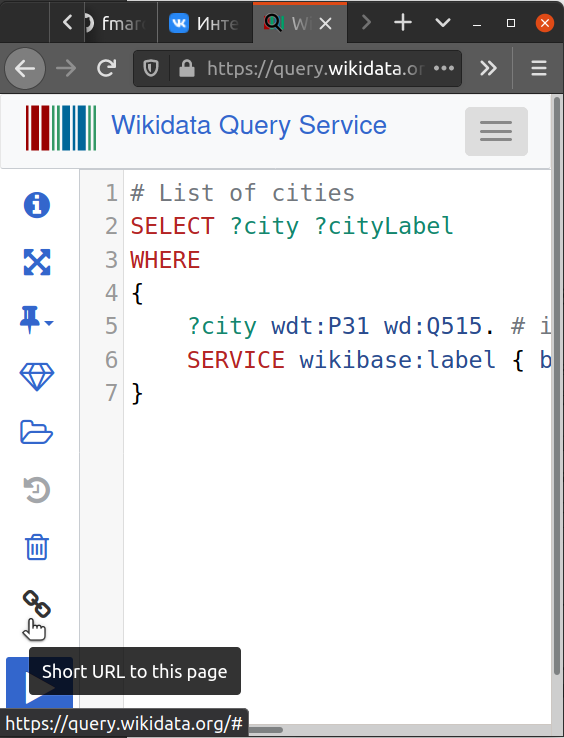
\includegraphics[width=\linewidth]{chapter/intro/WD_Query_Service_Short_URL_2020.png}}
    }
	\caption{The chain symbol button creates a short link to the SPARQL script, Wikidata Query Service, 2020.}
	\labfig{fig:WDQS-Short-URL-creation}
\end{marginfigure}

The Wikidata Query Service is shown in~\reffig{fig:WDQS-Short-URL-creation}. 
The bottom button with a chain symbol allows you to create a short link to the SPARQL script. 

See question on page~\pageref{question:short-link-to-SPARQL}.



\section{Aircraft from small to large}
\labsec{answer-aircraft}

\begin{exercise}%
    \label{answer:formulate-your-short-label-for-question-here-please}
Question one?
\end{exercise}

Answer text.



\section{From towns to cities with millions of inhabitants}
\labsec{answer-towns}

\begin{exercise}%
    \label{answer:formulate-your-short-label-for-question-here-please2}
Question two?
\end{exercise}

Answer text.


\section{Programming languages and its creators}
\labsec{answer-languages}
\begin{exercise}
    \label{answer:prog_lang_1}
Correlate a programming language and its developer.
\newline
	\begin{tabular}{ll}
		Developer & Language\\
		\hline
		J. Ichbiah & \href{https://www.wikidata.org/wiki/Q154755}{Ada}\\
		C. Moore & \href{https://www.wikidata.org/wiki/Q275472}{Forth}\\
		J. Armstrong & \href{https://www.wikidata.org/wiki/Q334879}{Erlang}\\
	\end{tabular}
\end{exercise}
    The Ada programming language was developed by Jean Ichbiah, Forth was developed by Charles H. Moore, and the creator of Erlang is believed to be Joe Armstrong. The answer to the question can also be obtained by running the following SPARQL query (listing \ref{lst:prog_lang_answer_1}). 
	\begin{lstlisting}[language=SPARQL, caption={{Programming languages developers}\protect\footnotemark}, label=lst:prog_lang_answer_1]
		SELECT ?item_label ?developer_label
		WHERE
		{
		 ?item wdt:P31 wd:Q9143
		 ; rdfs:label ?item_label. 
		 ?item wdt:P178 ?developer.
		 ?developer rdfs:label ?developer_label.
		 
		 FILTER (LANG(?item_label) = "en"). 
		 FILTER (LANG(?developer_label) = "en"). 
		}
		ORDER BY DESC (?item_label)
	\end{lstlisting}
SPARQL query: \href{https://w.wiki/kfZ}{https://w.wiki/kfZ}
\newline
Question from page~\pageref{question:prog_lang_1}.


\begin{exercise}
    \label{answer:prog_lang_2}
Which image is the programming language logo \href{https://www.wikidata.org/wiki/Q513238}{LOLCODE}: \newline
	\begin{tabular}{c c c c}

\includegraphics[width=2cm]{./chapter/programming_language/task_2_logo_1.PNG} & 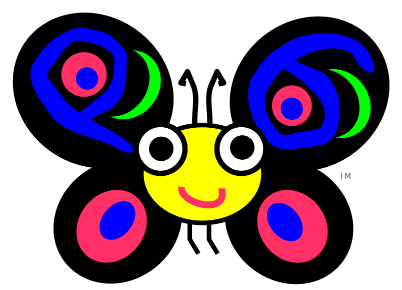
\includegraphics[width=2cm]{./chapter/programming_language/task_2_logo_2.PNG} & 
\includegraphics[width=2cm]{./chapter/programming_language/task_2_logo_3.PNG} & 
\includegraphics[width=2cm]{./chapter/programming_language/task_2_logo_4.PNG}
	\end{tabular}
\end{exercise}
    The third picture is the logo of the LOLCODE programming language. The answer to the question can also be obtained by running the following SPARQL query (listing \ref{lst:prog_lang_answer_1}). 
	\begin{lstlisting}[language=SPARQL, caption={{Programmers languages logos}\protect\footnotemark}, label=lst:prog_lang_answer_1]
		#defaultView:ImageGrid
		SELECT ?item_label ?image
		WHERE
		{
		 ?item wdt:P31 wd:Q9143 # instances of programming language
		 ; rdfs:label ?item_label. 
		 ?item wdt:P154 ?image. # image
		 	
		 	FILTER (lang(?item_label) = "en")
}
	\end{lstlisting}
SPARQL query: \href{https://w.wiki/kfd}{https://w.wiki/kfd}
\newline
Question from page~\pageref{question:prog_lang_2}.


\begin{exercise}
    \label{answer:prog_lang_3}
Fill the gaps.\newline
\href{https://www.wikidata.org/wiki/Q83303}{Fortran} ranks first in terms of the number of its dialects. Their number reaches about \underline{\hspace{1cm}}. In second place is \href{https://www.wikidata.org/wiki/Q132874}{Lisp}, it has \underline{\hspace{1cm}} dialects. The third place is shared by\href{https://www.wikidata.org/wiki/Q597330}{Standard ML} and \href{https://www.wikidata.org/wiki/Q633894}{Object Pascal} with \underline{\hspace{1cm}} dialects.\newline
\end{exercise}
 It is believed that Fortran has 8 to 12 dialects, Lisp has 6 dialects, and Standard ML and Object Pascal have 3 dialects.
    
Question from page~\pageref{question:prog_lang_3}.

